\section{Results on BAliBASE datasets}
\label{sec:result_balibase}
%############################# RV20
\begin{figure*}[!htbp]
	\centering
	\begin{adjustwidth}{-1cm}{-1cm}
		\begin{subfigure}{0.22\textwidth}
			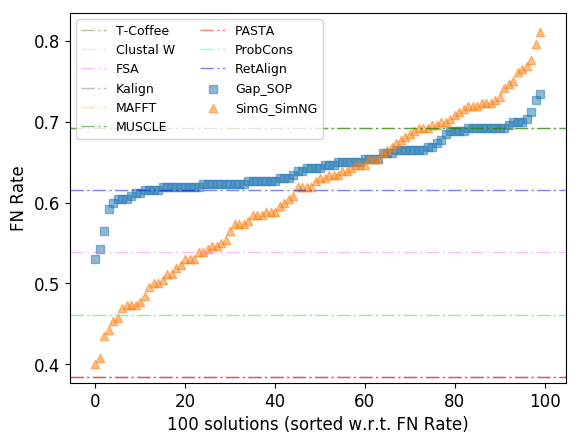
\includegraphics[width=\columnwidth]{Figure/summary/precomputedInit/Balibase/BB20001_fnrate_density_single_run}
			\caption{BB20001}
			%\label{fig:con_pr09}
		\end{subfigure}	
		\begin{subfigure}{0.22\textwidth}
			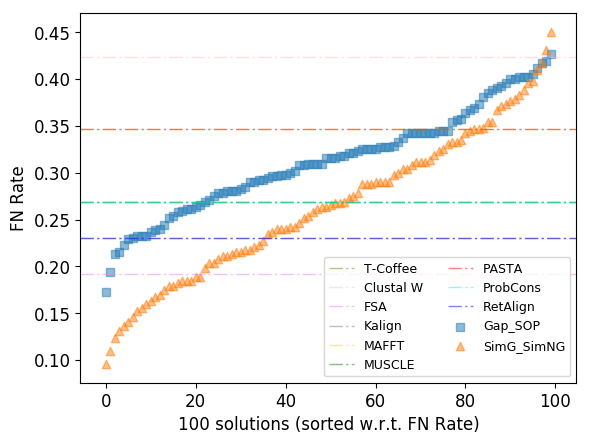
\includegraphics[width=\columnwidth]{Figure/summary/precomputedInit/Balibase/BB20010_fnrate_density_single_run}
			\caption{BB20010}
			%\label{fig:con_pr09}
		\end{subfigure}
		\begin{subfigure}{0.22\textwidth}
			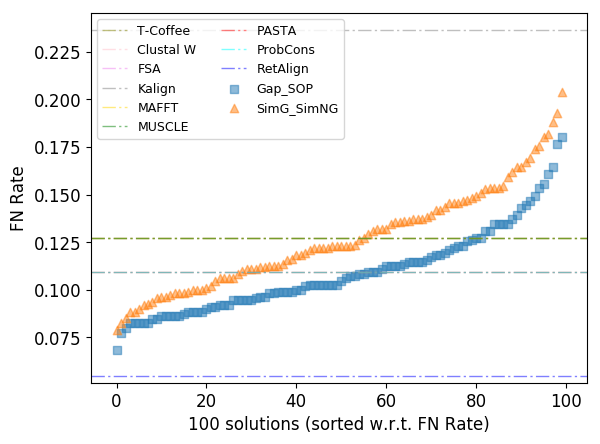
\includegraphics[width=\columnwidth]{Figure/summary/precomputedInit/Balibase/BB20022_fnrate_density_single_run}
			\caption{BB20022}
			%\label{fig:con_pr09}
		\end{subfigure}
		\begin{subfigure}{0.22\textwidth}
			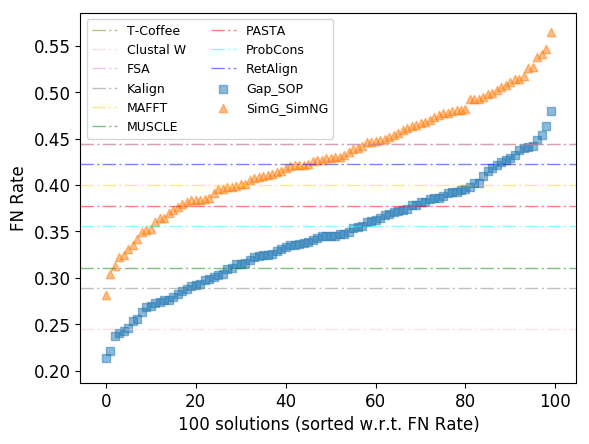
\includegraphics[width=\columnwidth]{Figure/summary/precomputedInit/Balibase/BB20033_fnrate_density_single_run}
			\caption{BB20033}
			%\label{fig:con_pr09}
		\end{subfigure}
		\begin{subfigure}{0.22\textwidth}
			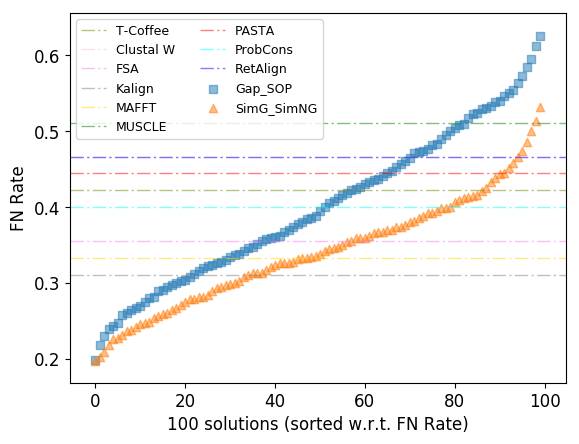
\includegraphics[width=\columnwidth]{Figure/summary/precomputedInit/Balibase/BB20041_fnrate_density_single_run}
			\caption{BB20041}
			%\label{fig:con_pr09}
		\end{subfigure}
		\begin{subfigure}{0.22\textwidth}
			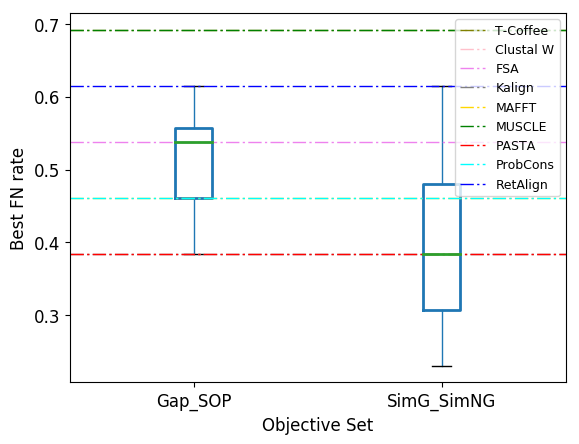
\includegraphics[width=\columnwidth]{Figure/summary/precomputedInit/Balibase/BB20001_objset_fnrate_rank}
			\caption{BB20001}
			%\label{fig:con_pr09}
		\end{subfigure}	
		\begin{subfigure}{0.22\textwidth}
			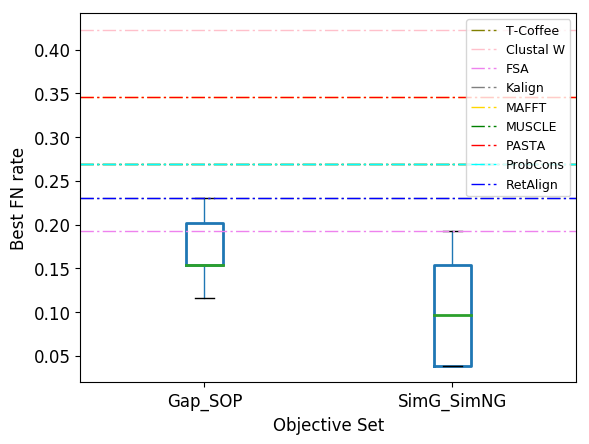
\includegraphics[width=\columnwidth]{Figure/summary/precomputedInit/Balibase/BB20010_objset_fnrate_rank}
			\caption{BB20010}
			%\label{fig:con_pr09}
		\end{subfigure}
		\begin{subfigure}{0.22\textwidth}
			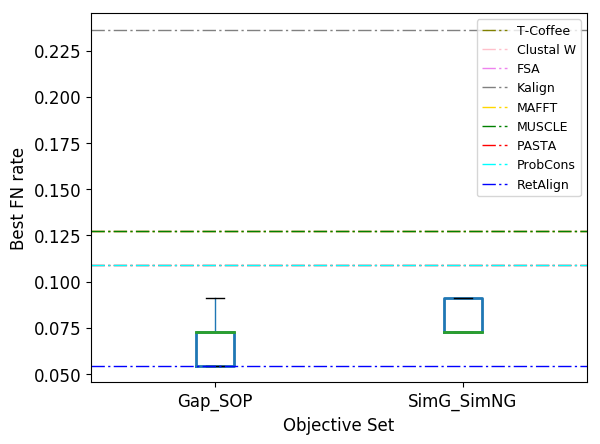
\includegraphics[width=\columnwidth]{Figure/summary/precomputedInit/Balibase/BB20022_objset_fnrate_rank}
			\caption{BB20022}
			%\label{fig:con_pr09}
		\end{subfigure}
		\begin{subfigure}{0.22\textwidth}
			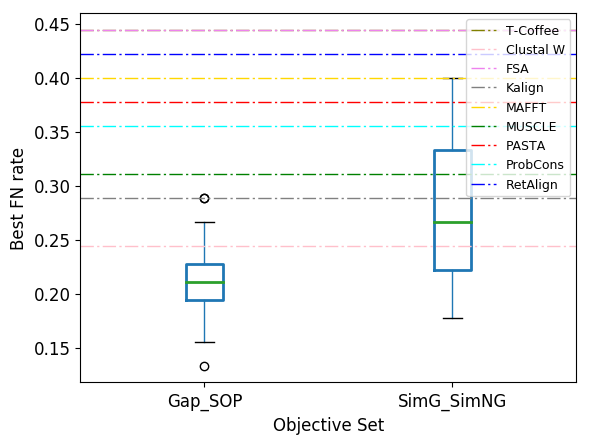
\includegraphics[width=\columnwidth]{Figure/summary/precomputedInit/Balibase/BB20033_objset_fnrate_rank}
			\caption{BB20033}
			%\label{fig:con_pr09}
		\end{subfigure}
		\begin{subfigure}{0.22\textwidth}
			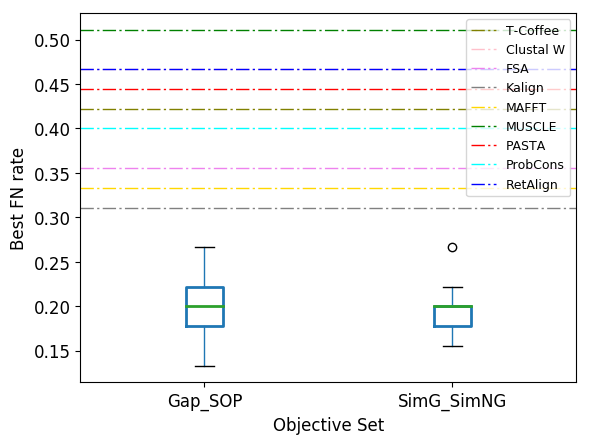
\includegraphics[width=\columnwidth]{Figure/summary/precomputedInit/Balibase/BB20041_objset_fnrate_rank}
			\caption{BB20041}
			%\label{fig:con_pr09}
		\end{subfigure}
		\caption{RV20: Top panel (part (a) - (d)) shows the FN rate of 100 final solutions averaged over 20 runs. At first, we sorted the FN rates of each solution set. Then we average the FN rates at each sorted position of all the sets. Bottom panel (part (e) - (h)) shows the distribution of the best FN rates collected from all runs. In each figure, the horizontal lines show the performance of the state-of-the-art tools.}
		\label{fig:rv20_fn_rate}
	\end{adjustwidth}
\end{figure*}


\begin{figure*}[!htbp]
	\centering
	\begin{adjustwidth}{-1cm}{-1cm}
		\begin{subfigure}{0.22\textwidth}
			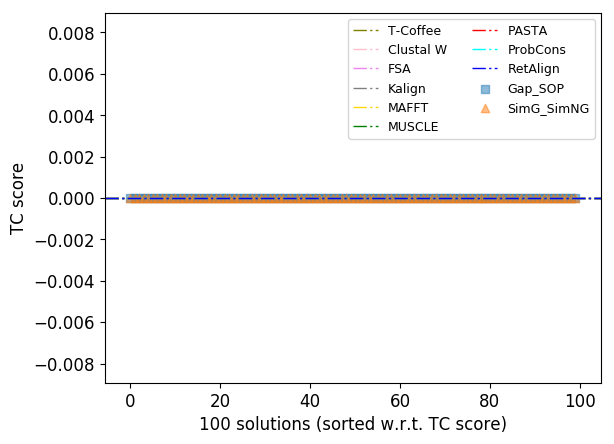
\includegraphics[width=\columnwidth]{Figure/summary/precomputedInit/Balibase/BB20001_tc_density_single_run_2}
			\caption{BB20001}
			%\label{fig:con_pr09}
		\end{subfigure}	
		\begin{subfigure}{0.22\textwidth}
			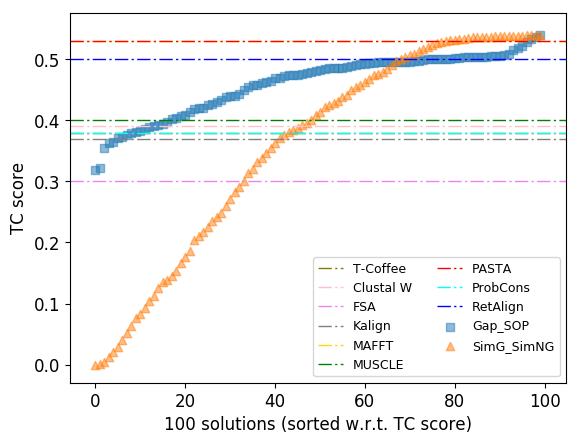
\includegraphics[width=\columnwidth]{Figure/summary/precomputedInit/Balibase/BB20010_tc_density_single_run_2}
			\caption{BB20010}
			%\label{fig:con_pr09}
		\end{subfigure}
		\begin{subfigure}{0.22\textwidth}
			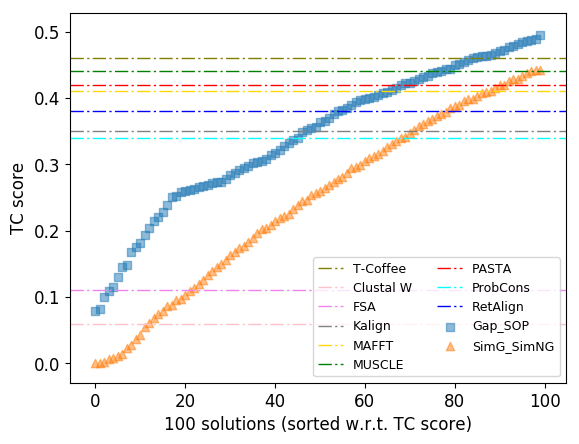
\includegraphics[width=\columnwidth]{Figure/summary/precomputedInit/Balibase/BB20022_tc_density_single_run_2}
			\caption{BB20022}
			%\label{fig:con_pr09}
		\end{subfigure}
		\begin{subfigure}{0.22\textwidth}
			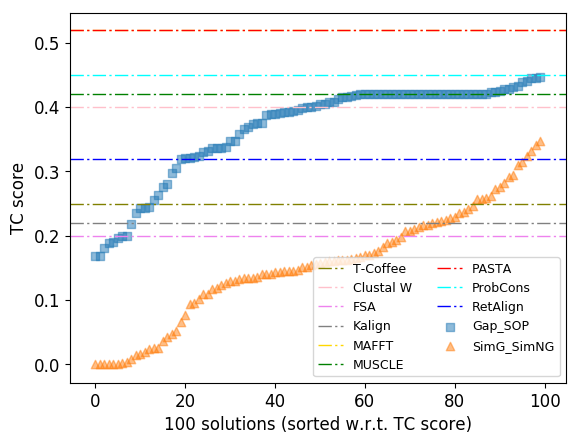
\includegraphics[width=\columnwidth]{Figure/summary/precomputedInit/Balibase/BB20033_tc_density_single_run_2}
			\caption{BB20033}
			%\label{fig:con_pr09}
		\end{subfigure}
		\begin{subfigure}{0.22\textwidth}
			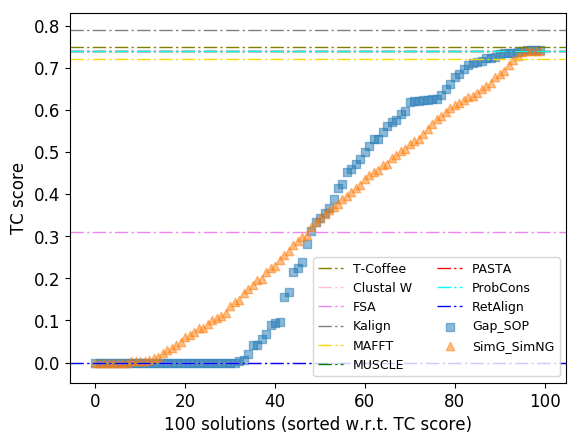
\includegraphics[width=\columnwidth]{Figure/summary/precomputedInit/Balibase/BB20041_tc_density_single_run_2}
			\caption{BB20041}
			%\label{fig:con_pr09}
		\end{subfigure}
		\begin{subfigure}{0.22\textwidth}
			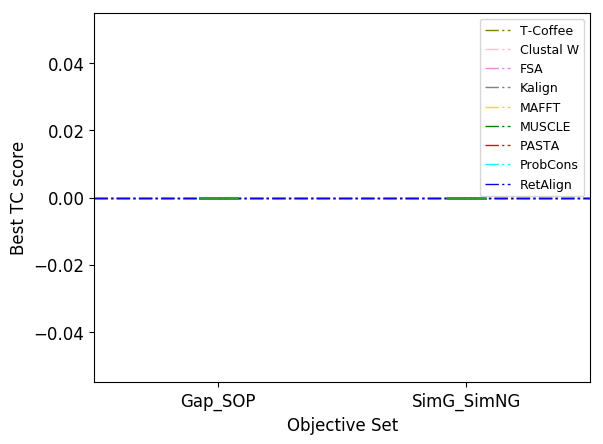
\includegraphics[width=\columnwidth]{Figure/summary/precomputedInit/Balibase/BB20001_objset_tc_rank_2}
			\caption{BB20001}
			%\label{fig:con_pr09}
		\end{subfigure}	
		\begin{subfigure}{0.22\textwidth}
			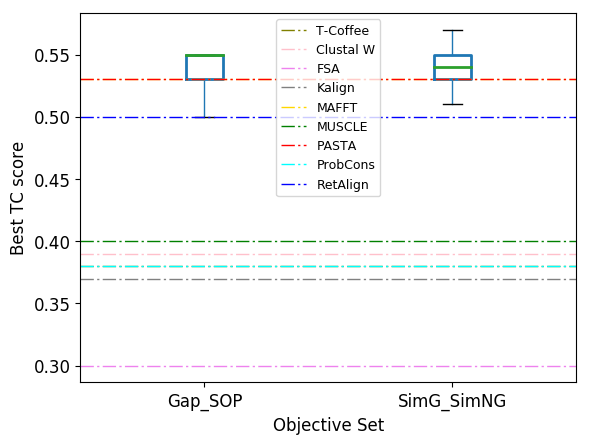
\includegraphics[width=\columnwidth]{Figure/summary/precomputedInit/Balibase/BB20010_objset_tc_rank_2}
			\caption{BB20010}
			%\label{fig:con_pr09}
		\end{subfigure}
		\begin{subfigure}{0.22\textwidth}
			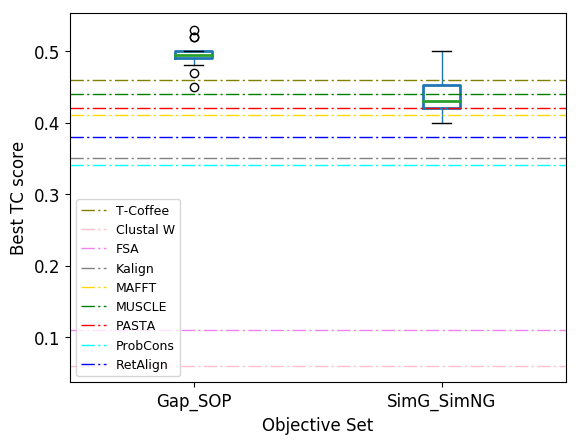
\includegraphics[width=\columnwidth]{Figure/summary/precomputedInit/Balibase/BB20022_objset_tc_rank_2}
			\caption{BB20022}
			%\label{fig:con_pr09}
		\end{subfigure}
		\begin{subfigure}{0.22\textwidth}
			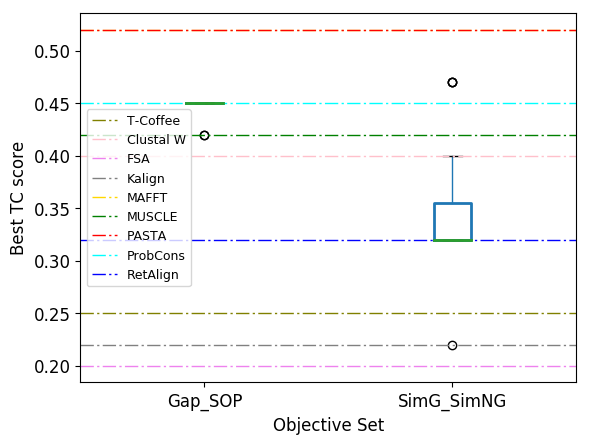
\includegraphics[width=\columnwidth]{Figure/summary/precomputedInit/Balibase/BB20033_objset_tc_rank_2}
			\caption{BB20033}
			%\label{fig:con_pr09}
		\end{subfigure}
		\begin{subfigure}{0.22\textwidth}
			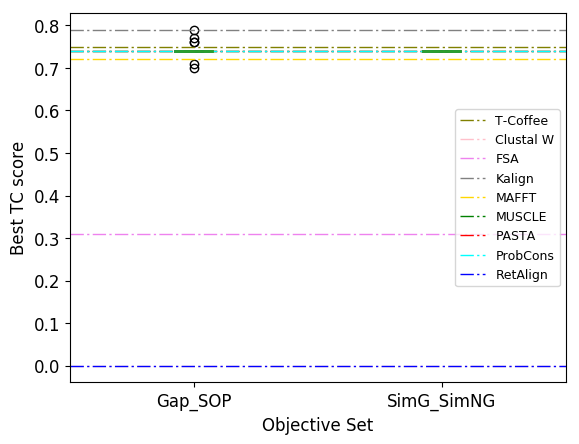
\includegraphics[width=\columnwidth]{Figure/summary/precomputedInit/Balibase/BB20041_objset_tc_rank_2}
			\caption{BB20041}
			%\label{fig:con_pr09}
		\end{subfigure}
		\caption{RV20: Top panel (part (a) - (e)) shows the TC score of 100 final solutions averaged over 20 runs. At first, we sorted the TC scores of each solution set. Then we average the TC scores at each sorted position of all the sets. Bottom panel (part (f) - (j)) shows the distribution of the best TC scores collected from all runs. In each figure, the horizontal lines show the performance of the state-of-the-art tools.}
		\label{fig:rv20_tc}
	\end{adjustwidth}
\end{figure*}

\begin{figure*}[!htbp]
	\centering
	\begin{adjustwidth}{-1cm}{-1cm}
		\begin{subfigure}{0.22\textwidth}
			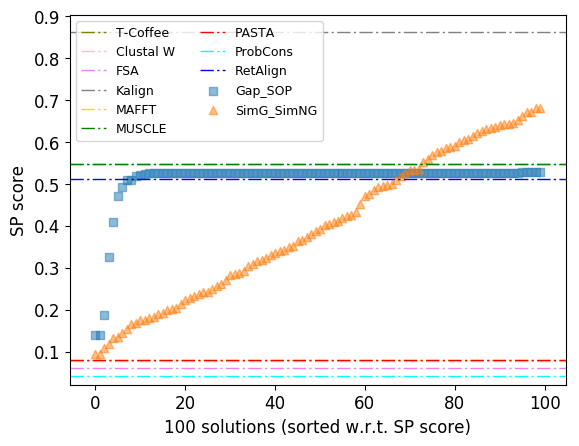
\includegraphics[width=\columnwidth]{Figure/summary/precomputedInit/Balibase/BB20001_pairs_density_single_run_2}
			\caption{BB20001}
			%\label{fig:con_pr09}
		\end{subfigure}	
		\begin{subfigure}{0.22\textwidth}
			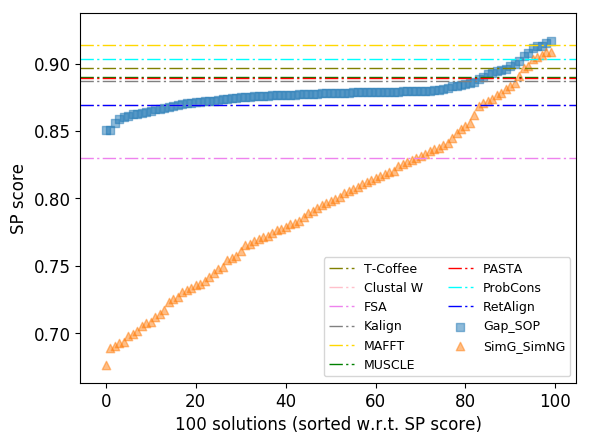
\includegraphics[width=\columnwidth]{Figure/summary/precomputedInit/Balibase/BB20010_pairs_density_single_run_2}
			\caption{BB20010}
			%\label{fig:con_pr09}
		\end{subfigure}
		\begin{subfigure}{0.22\textwidth}
			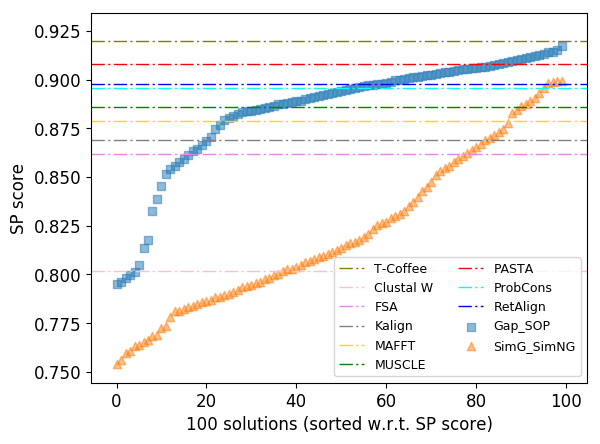
\includegraphics[width=\columnwidth]{Figure/summary/precomputedInit/Balibase/BB20022_pairs_density_single_run_2}
			\caption{BB20022}
			%\label{fig:con_pr09}
		\end{subfigure}
		\begin{subfigure}{0.22\textwidth}
			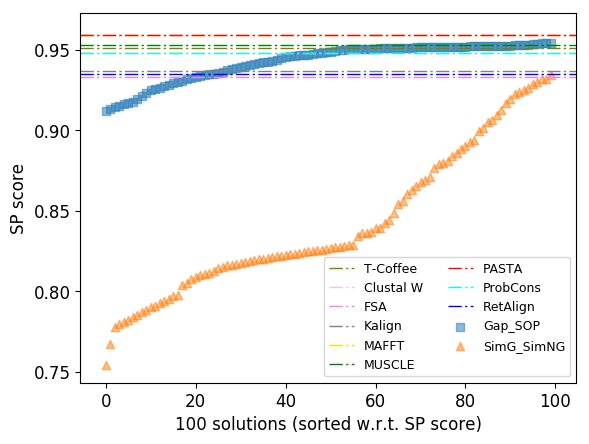
\includegraphics[width=\columnwidth]{Figure/summary/precomputedInit/Balibase/BB20033_pairs_density_single_run_2}
			\caption{BB20033}
			%\label{fig:con_pr09}
		\end{subfigure}
		\begin{subfigure}{0.22\textwidth}
			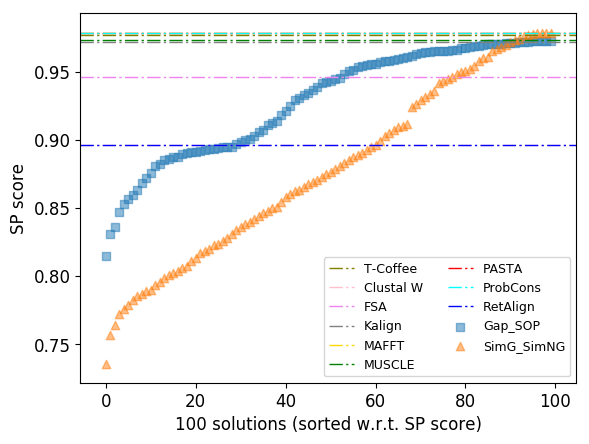
\includegraphics[width=\columnwidth]{Figure/summary/precomputedInit/Balibase/BB20041_pairs_density_single_run_2}
			\caption{BB20041}
			%\label{fig:con_pr09}
		\end{subfigure}
		\begin{subfigure}{0.22\textwidth}
			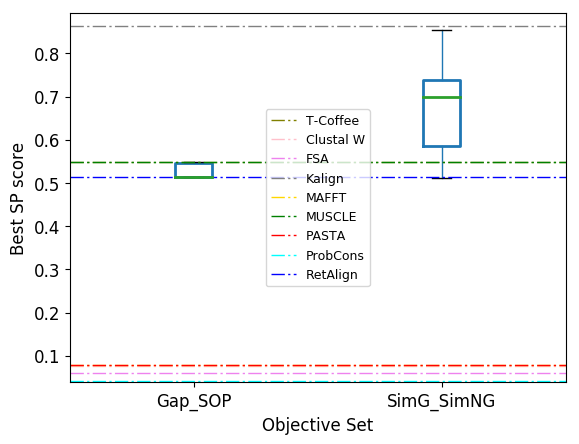
\includegraphics[width=\columnwidth]{Figure/summary/precomputedInit/Balibase/BB20001_objset_pairs_rank_2}
			\caption{BB20001}
			%\label{fig:con_pr09}
		\end{subfigure}	
		\begin{subfigure}{0.22\textwidth}
			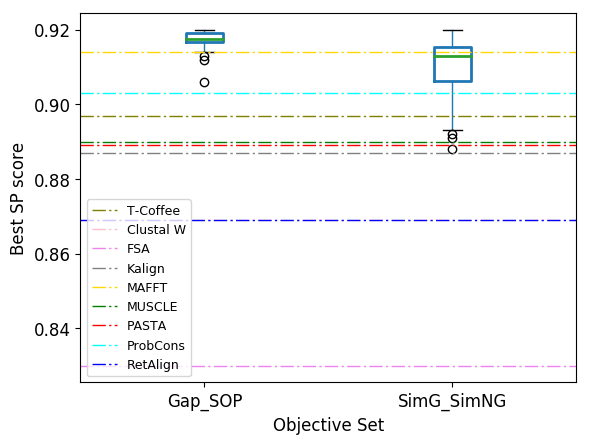
\includegraphics[width=\columnwidth]{Figure/summary/precomputedInit/Balibase/BB20010_objset_pairs_rank_2}
			\caption{BB20010}
			%\label{fig:con_pr09}
		\end{subfigure}
		\begin{subfigure}{0.22\textwidth}
			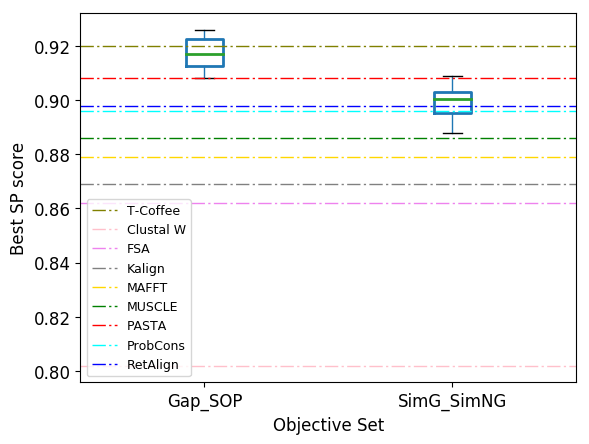
\includegraphics[width=\columnwidth]{Figure/summary/precomputedInit/Balibase/BB20022_objset_pairs_rank_2}
			\caption{BB20022}
			%\label{fig:con_pr09}
		\end{subfigure}
		\begin{subfigure}{0.22\textwidth}
			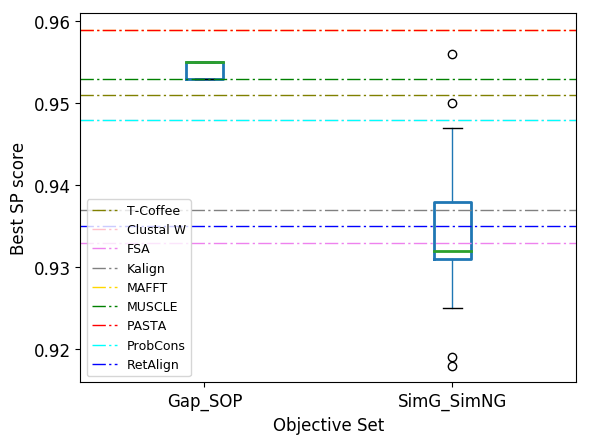
\includegraphics[width=\columnwidth]{Figure/summary/precomputedInit/Balibase/BB20033_objset_pairs_rank_2}
			\caption{BB20033}
			%\label{fig:con_pr09}
		\end{subfigure}
		\begin{subfigure}{0.22\textwidth}
			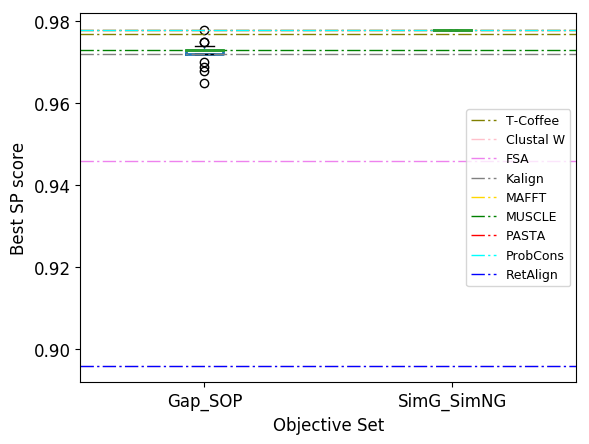
\includegraphics[width=\columnwidth]{Figure/summary/precomputedInit/Balibase/BB20041_objset_pairs_rank_2}
			\caption{BB20041}
			%\label{fig:con_pr09}
		\end{subfigure}
		\caption{RV20: Top panel (part (a) - (e)) shows the SP score of 100 final solutions averaged over 20 runs. At first, we sorted the SP scores of each solution set. Then we average the SP scores at each sorted position of all the sets. Bottom panel (part (f) - (j)) shows the distribution of the best SP scores collected from all runs. In each figure, the horizontal lines show the performance of the state-of-the-art tools.}
		\label{fig:rv20_sp}
	\end{adjustwidth}
\end{figure*}


\begin{figure*}[!htbp]
	\centering
	\begin{adjustwidth}{-1cm}{-1cm}
		\begin{subfigure}{0.22\textwidth}
			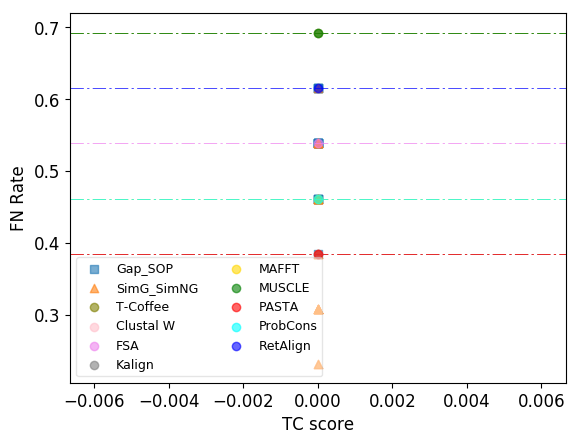
\includegraphics[width=\columnwidth]{Figure/summary/precomputedInit/Balibase/BB20001_fnrate_vs_tc_2}
			\caption{BB20001}
			%\label{fig:con_pr09}
		\end{subfigure}	
		\begin{subfigure}{0.22\textwidth}
			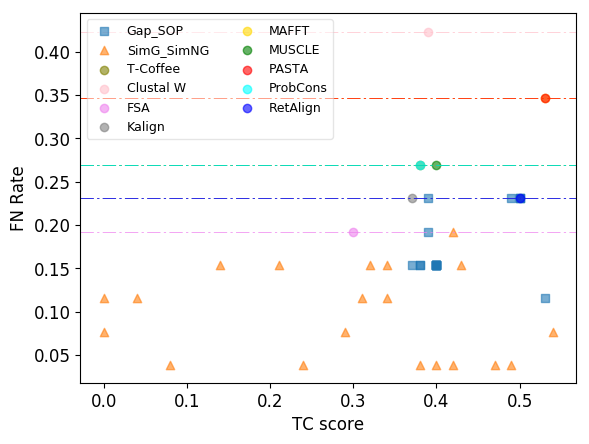
\includegraphics[width=\columnwidth]{Figure/summary/precomputedInit/Balibase/BB20010_fnrate_vs_tc_2}
			\caption{BB20010}
			%\label{fig:con_pr09}
		\end{subfigure}
		\begin{subfigure}{0.22\textwidth}
			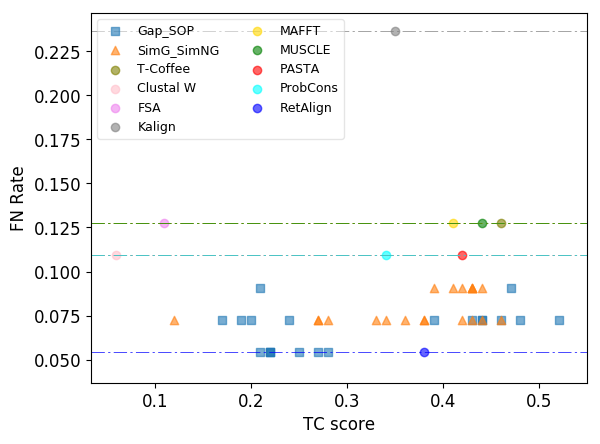
\includegraphics[width=\columnwidth]{Figure/summary/precomputedInit/Balibase/BB20022_fnrate_vs_tc_2}
			\caption{BB20022}
			%\label{fig:con_pr09}
		\end{subfigure}
		\begin{subfigure}{0.22\textwidth}
			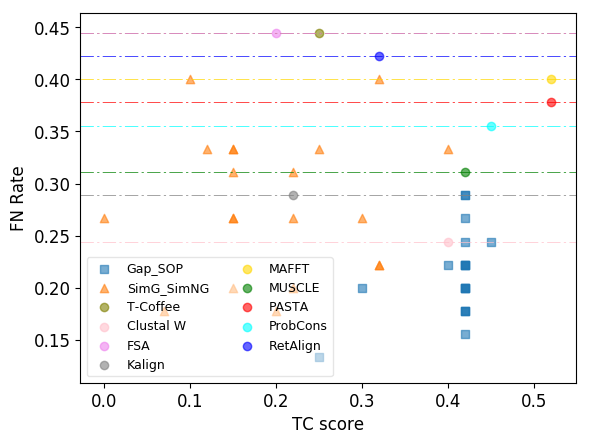
\includegraphics[width=\columnwidth]{Figure/summary/precomputedInit/Balibase/BB20033_fnrate_vs_tc_2}
			\caption{BB20033}
			%\label{fig:con_pr09}
		\end{subfigure}	
		\begin{subfigure}{0.22\textwidth}
			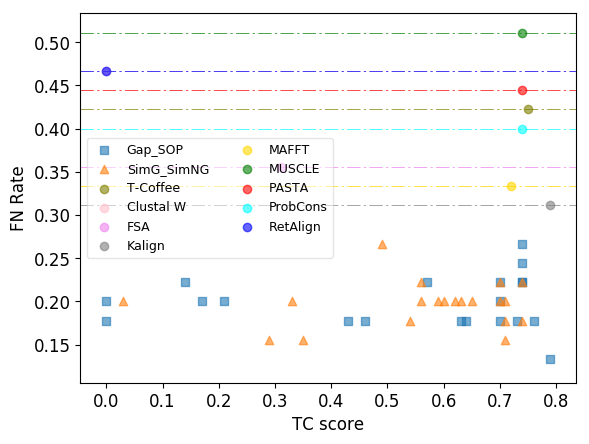
\includegraphics[width=\columnwidth]{Figure/summary/precomputedInit/Balibase/BB20041_fnrate_vs_tc_2}
			\caption{BB20041}
			%\label{fig:con_pr09}
		\end{subfigure}
		%%%%%%%%%%
		\begin{subfigure}{0.22\textwidth}
			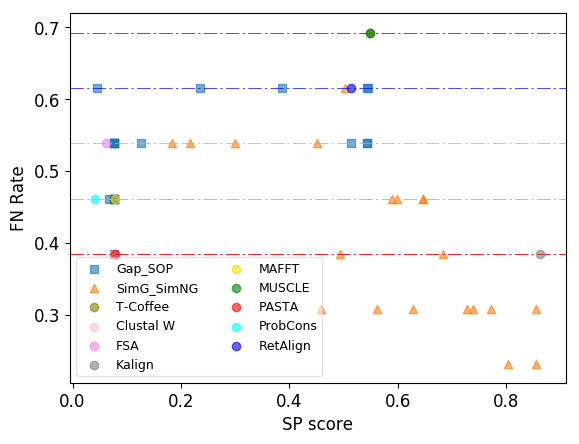
\includegraphics[width=\columnwidth]{Figure/summary/precomputedInit/Balibase/BB20001_fnrate_vs_sp_2}
			\caption{BB20001}
			%\label{fig:con_pr09}
		\end{subfigure}	
		\begin{subfigure}{0.22\textwidth}
			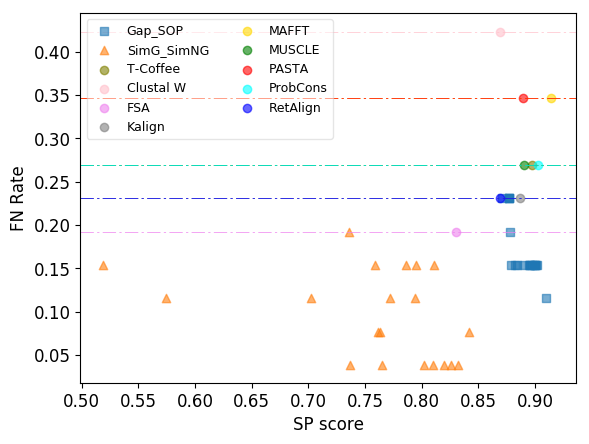
\includegraphics[width=\columnwidth]{Figure/summary/precomputedInit/Balibase/BB20010_fnrate_vs_sp_2}
			\caption{BB20010}
			%\label{fig:con_pr09}
		\end{subfigure}
		\begin{subfigure}{0.22\textwidth}
			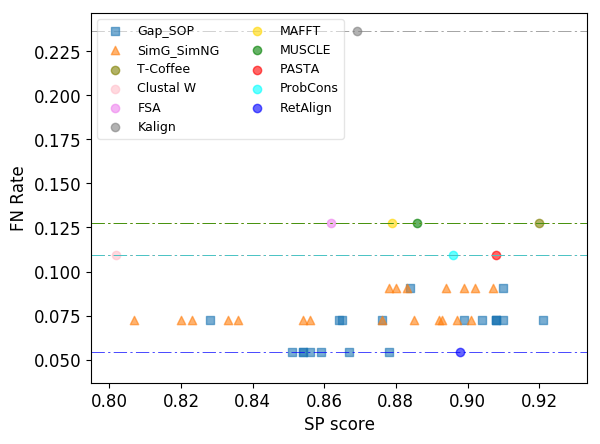
\includegraphics[width=\columnwidth]{Figure/summary/precomputedInit/Balibase/BB20022_fnrate_vs_sp_2}
			\caption{BB20022}
			%\label{fig:con_pr09}
		\end{subfigure}
		\begin{subfigure}{0.22\textwidth}
			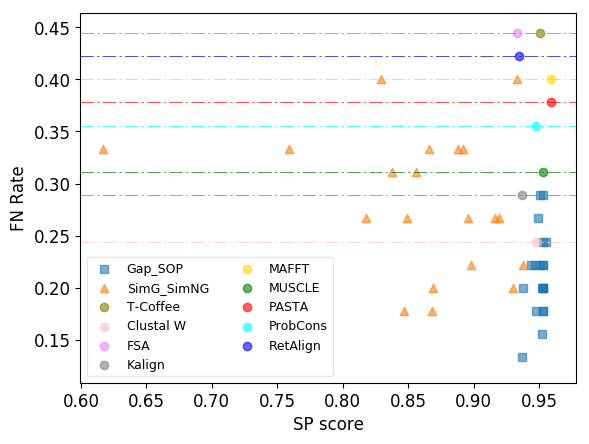
\includegraphics[width=\columnwidth]{Figure/summary/precomputedInit/Balibase/BB20033_fnrate_vs_sp_2}
			\caption{BB20033}
			%\label{fig:con_pr09}
		\end{subfigure}	
		\begin{subfigure}{0.22\textwidth}
			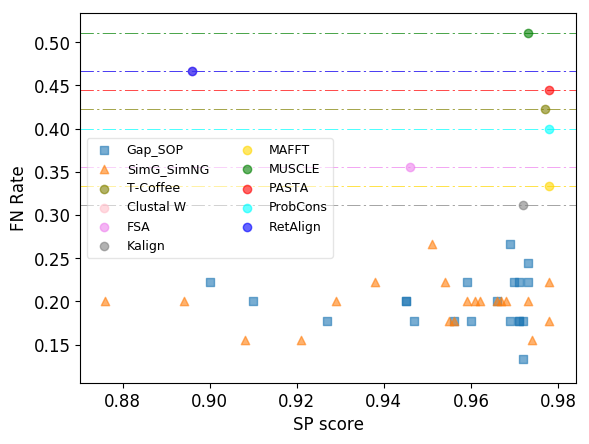
\includegraphics[width=\columnwidth]{Figure/summary/precomputedInit/Balibase/BB20041_fnrate_vs_sp_2}
			\caption{BB20041}
			%\label{fig:con_pr09}
		\end{subfigure}
		\caption{RV20: Top panel (part (a) - (e)) shows the relationship between FN rate and TC score for different alignments. And bottom panel (part (f) - (j)) shows the relationship between FN rate and SP score. The horizontal lines mark the FN rates achieved by the state-of-the-art tools.}
		\label{fig:rv20_fnrate_vs_tc}
	\end{adjustwidth}
\end{figure*}
%############################# RV30
\begin{figure*}[!htbp]
	
	\begin{adjustwidth}{-1cm}{-1cm}
		\centering
		\begin{subfigure}{0.22\textwidth}
			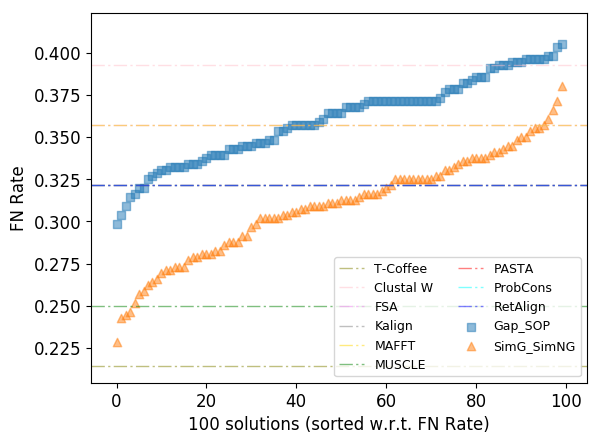
\includegraphics[width=\columnwidth]{Figure/summary/precomputedInit/Balibase/BB30002_fnrate_density_single_run}
			\caption{BB30002}
			%\label{fig:con_pr09}
		\end{subfigure}	
		\begin{subfigure}{0.22\textwidth}
			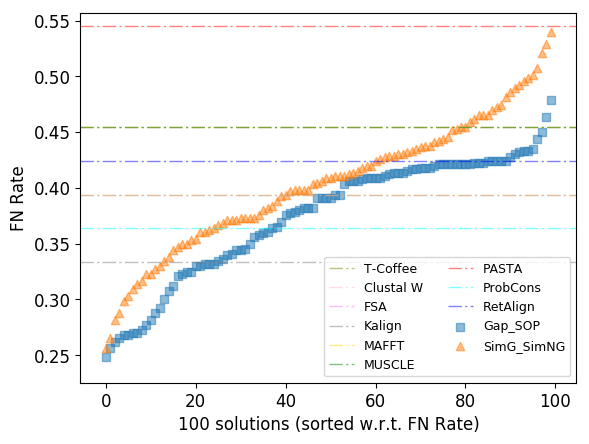
\includegraphics[width=\columnwidth]{Figure/summary/precomputedInit/Balibase/BB30008_fnrate_density_single_run}
			\caption{BB30008}
			%\label{fig:con_pr09}
		\end{subfigure}
		\begin{subfigure}{0.22\textwidth}
			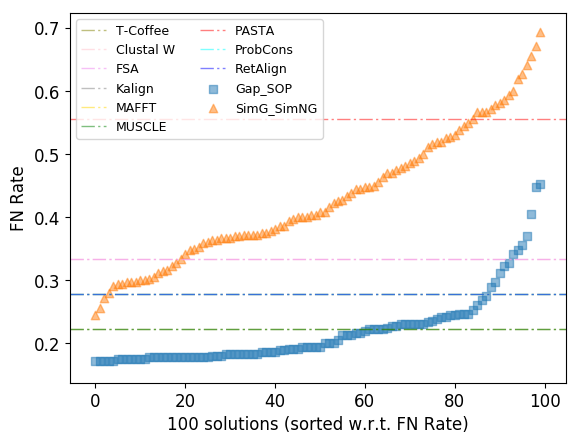
\includegraphics[width=\columnwidth]{Figure/summary/precomputedInit/Balibase/BB30015_fnrate_density_single_run}
			\caption{BB30015}
			%\label{fig:con_pr09}
		\end{subfigure}
		\begin{subfigure}{0.22\textwidth}
			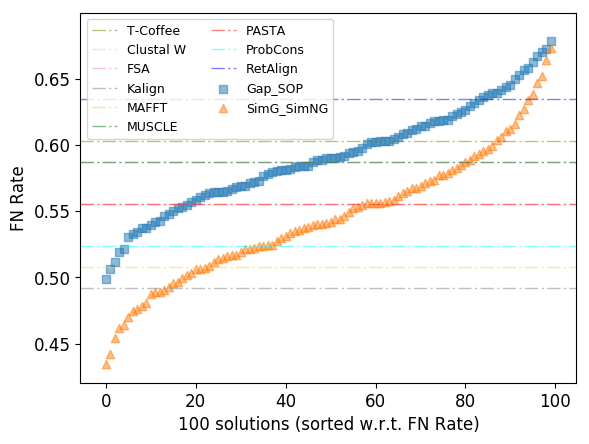
\includegraphics[width=\columnwidth]{Figure/summary/precomputedInit/Balibase/BB30022_fnrate_density_single_run}
			\caption{BB30022}
			%\label{fig:con_pr09}
		\end{subfigure}
		\begin{subfigure}{0.22\textwidth}
			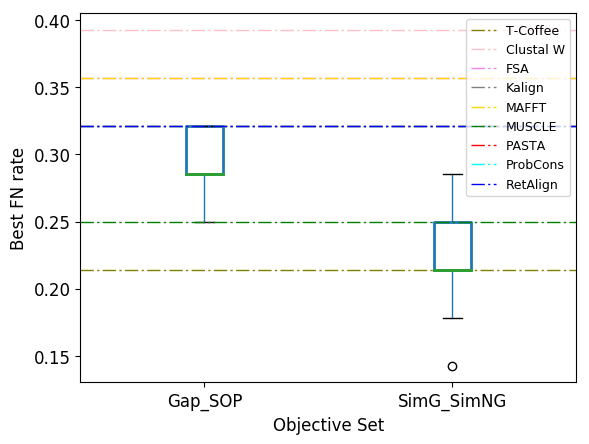
\includegraphics[width=\columnwidth]{Figure/summary/precomputedInit/Balibase/BB30002_objset_fnrate_rank}
			\caption{BB30002}
			%\label{fig:con_pr09}
		\end{subfigure}
		\begin{subfigure}{0.22\textwidth}
			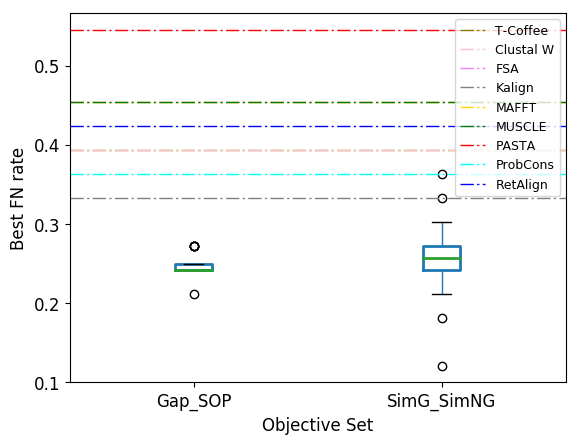
\includegraphics[width=\columnwidth]{Figure/summary/precomputedInit/Balibase/BB30008_objset_fnrate_rank}
			\caption{BB30008}
			%\label{fig:con_pr09}
		\end{subfigure}		
		\begin{subfigure}{0.22\textwidth}
			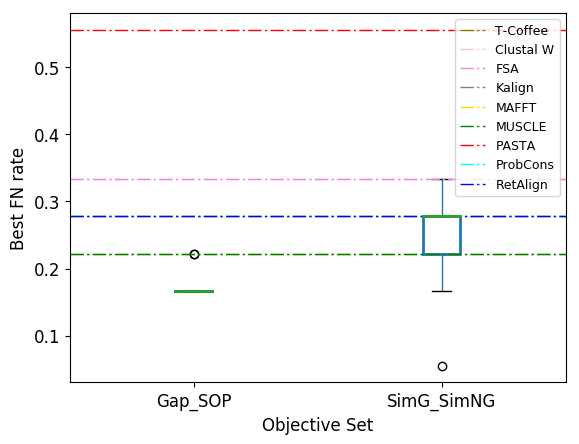
\includegraphics[width=\columnwidth]{Figure/summary/precomputedInit/Balibase/BB30015_objset_fnrate_rank}
			\caption{BB30015}
			%\label{fig:con_pr09}
		\end{subfigure}
		\begin{subfigure}{0.22\textwidth}
			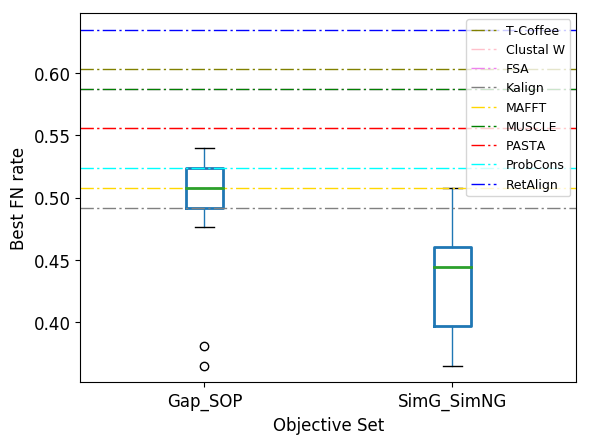
\includegraphics[width=\columnwidth]{Figure/summary/precomputedInit/Balibase/BB30022_objset_fnrate_rank}
			\caption{BB30022}
			%\label{fig:con_pr09}
		\end{subfigure}
		\caption{RV30: Top panel (part (a) - (d)) shows the FN rate of 100 final solutions averaged over 20 runs. At first, we sorted the FN rates of each solution set. Then we average the FN rates at each sorted position of all the sets. Bottom panel (part (e) - (h)) shows the distribution of the best FN rates collected from all runs. In each figure, the horizontal lines show the performance of the state-of-the-art tools.}
		\label{fig:rv30_fn_rate}
	\end{adjustwidth}
\end{figure*}


\begin{figure*}[!htbp]
	
	\begin{adjustwidth}{-1cm}{-1cm}
		\centering
		\begin{subfigure}{0.22\textwidth}
			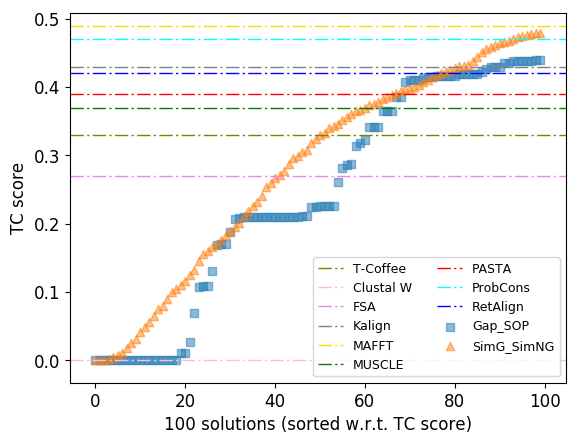
\includegraphics[width=\columnwidth]{Figure/summary/precomputedInit/Balibase/BB30002_tc_density_single_run_2}
			\caption{BB30002}
			%\label{fig:con_pr09}
		\end{subfigure}	
		\begin{subfigure}{0.22\textwidth}
			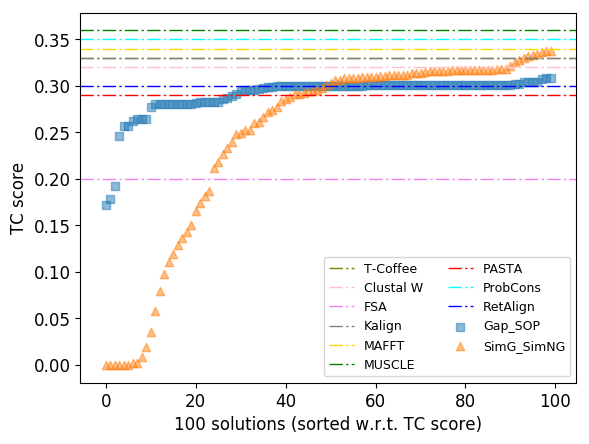
\includegraphics[width=\columnwidth]{Figure/summary/precomputedInit/Balibase/BB30008_tc_density_single_run_2}
			\caption{BB30008}
			%\label{fig:con_pr09}
		\end{subfigure}
		\begin{subfigure}{0.22\textwidth}
			\includegraphics[width=\columnwidth]{Figure/summary/precomputedInit/Balibase/BB30015_tc_density_single_run_2}
			\caption{BB30015}
			%\label{fig:con_pr09}
		\end{subfigure}
		\begin{subfigure}{0.22\textwidth}
			\includegraphics[width=\columnwidth]{Figure/summary/precomputedInit/Balibase/BB30022_tc_density_single_run_2}
			\caption{BB30022}
			%\label{fig:con_pr09}
		\end{subfigure}
		\begin{subfigure}{0.22\textwidth}
			\includegraphics[width=\columnwidth]{Figure/summary/precomputedInit/Balibase/BB30002_objset_tc_rank_2}
			\caption{BB30002}
			%\label{fig:con_pr09}
		\end{subfigure}	
		\begin{subfigure}{0.22\textwidth}
			\includegraphics[width=\columnwidth]{Figure/summary/precomputedInit/Balibase/BB30008_objset_tc_rank_2}
			\caption{BB30008}
			%\label{fig:con_pr09}
		\end{subfigure}
		\begin{subfigure}{0.22\textwidth}
			\includegraphics[width=\columnwidth]{Figure/summary/precomputedInit/Balibase/BB30015_objset_tc_rank_2}
			\caption{BB30015}
			%\label{fig:con_pr09}
		\end{subfigure}
		\begin{subfigure}{0.22\textwidth}
			\includegraphics[width=\columnwidth]{Figure/summary/precomputedInit/Balibase/BB30022_objset_tc_rank_2}
			\caption{BB30022}
			%\label{fig:con_pr09}
		\end{subfigure}
		\caption{RV30: Top panel (part (a) - (d)) shows the TC score of 100 final solutions averaged over 20 runs. At first, we sorted the TC scores of each solution set. Then we average the TC scores at each sorted position of all the sets. Bottom panel (part (e) - (h)) shows the distribution of the best TC scores collected from all runs. In each figure, the horizontal lines show the performance of the state-of-the-art tools.}
		\label{fig:rv30_tc}
	\end{adjustwidth}
\end{figure*}

\begin{figure*}[!htbp]
	
	\begin{adjustwidth}{-1cm}{-1cm}
		\centering
		\begin{subfigure}{0.22\textwidth}
			\includegraphics[width=\columnwidth]{Figure/summary/precomputedInit/Balibase/BB30002_pairs_density_single_run_2}
			\caption{BB30002}
			%\label{fig:con_pr09}
		\end{subfigure}	
		\begin{subfigure}{0.22\textwidth}
			\includegraphics[width=\columnwidth]{Figure/summary/precomputedInit/Balibase/BB30008_pairs_density_single_run_2}
			\caption{BB30008}
			%\label{fig:con_pr09}
		\end{subfigure}
		\begin{subfigure}{0.22\textwidth}
			\includegraphics[width=\columnwidth]{Figure/summary/precomputedInit/Balibase/BB30015_pairs_density_single_run_2}
			\caption{BB30015}
			%\label{fig:con_pr09}
		\end{subfigure}
		\begin{subfigure}{0.22\textwidth}
			\includegraphics[width=\columnwidth]{Figure/summary/precomputedInit/Balibase/BB30022_pairs_density_single_run_2}
			\caption{BB30022}
			%\label{fig:con_pr09}
		\end{subfigure}
		\begin{subfigure}{0.22\textwidth}
			\includegraphics[width=\columnwidth]{Figure/summary/precomputedInit/Balibase/BB30002_objset_pairs_rank_2}
			\caption{BB30002}
			%\label{fig:con_pr09}
		\end{subfigure}	
		\begin{subfigure}{0.22\textwidth}
			\includegraphics[width=\columnwidth]{Figure/summary/precomputedInit/Balibase/BB30008_objset_pairs_rank_2}
			\caption{BB30008}
			%\label{fig:con_pr09}
		\end{subfigure}
		\begin{subfigure}{0.22\textwidth}
			\includegraphics[width=\columnwidth]{Figure/summary/precomputedInit/Balibase/BB30015_objset_pairs_rank_2}
			\caption{BB30015}
			%\label{fig:con_pr09}
		\end{subfigure}
		\begin{subfigure}{0.22\textwidth}
			\includegraphics[width=\columnwidth]{Figure/summary/precomputedInit/Balibase/BB30022_objset_pairs_rank_2}
			\caption{BB30022}
			%\label{fig:con_pr09}
		\end{subfigure}
		\caption{RV30: Top panel (part (a) - (d)) shows the SP score of 100 final solutions averaged over 20 runs. At first, we sorted the SP scores of each solution set. Then we average the SP scores at each sorted position of all the sets. Bottom panel (part (e) - (h)) shows the distribution of the best SP scores collected from all runs. In each figure, the horizontal lines show the performance of the state-of-the-art tools.}
		\label{fig:rv30_sp}
	\end{adjustwidth}
\end{figure*}


\begin{figure*}[!htbp]
	
	\begin{adjustwidth}{-1cm}{-1cm}
		\centering
		\begin{subfigure}{0.22\textwidth}
			\includegraphics[width=\columnwidth]{Figure/summary/precomputedInit/Balibase/BB30002_fnrate_vs_tc_2}
			\caption{BB30002}
			%\label{fig:con_pr09}
		\end{subfigure}	
		\begin{subfigure}{0.22\textwidth}
			\includegraphics[width=\columnwidth]{Figure/summary/precomputedInit/Balibase/BB30008_fnrate_vs_tc_2}
			\caption{BB30008}
			%\label{fig:con_pr09}
		\end{subfigure}
		\begin{subfigure}{0.22\textwidth}
			\includegraphics[width=\columnwidth]{Figure/summary/precomputedInit/Balibase/BB30015_fnrate_vs_tc_2}
			\caption{BB30015}
			%\label{fig:con_pr09}
		\end{subfigure}
		\begin{subfigure}{0.22\textwidth}
			\includegraphics[width=\columnwidth]{Figure/summary/precomputedInit/Balibase/BB30022_fnrate_vs_tc_2}
			\caption{BB30022}
			%\label{fig:con_pr09}
		\end{subfigure}	
		\caption{RV30: Top panel (part (a) - (d)) shows the relationship between FN rate and TC score for different alignments. And bottom panel (part (e) - (h)) shows the relationship between FN rate and SP score. The horizontal lines mark the FN rates achieved by the state-of-the-art tools.}
		\label{fig:rv30_fnrate_vs_tc}
	\end{adjustwidth}
\end{figure*}
%############################# RV40
\begin{figure*}[!htbp]
	\centering
	\begin{adjustwidth}{-1cm}{-1cm}
		\begin{subfigure}{0.22\textwidth}
			\includegraphics[width=\columnwidth]{Figure/summary/precomputedInit/Balibase/BB40001_fnrate_density_single_run}
			\caption{BB40001}
			%\label{fig:con_pr09}
		\end{subfigure}	
		\begin{subfigure}{0.22\textwidth}
			\includegraphics[width=\columnwidth]{Figure/summary/precomputedInit/Balibase/BB40013_fnrate_density_single_run}
			\caption{BB40013}
			%\label{fig:con_pr09}
		\end{subfigure}
		\begin{subfigure}{0.22\textwidth}
			\includegraphics[width=\columnwidth]{Figure/summary/precomputedInit/Balibase/BB40025_fnrate_density_single_run}
			\caption{BB40025}
			%\label{fig:con_pr09}
		\end{subfigure}
		\begin{subfigure}{0.22\textwidth}
			\includegraphics[width=\columnwidth]{Figure/summary/precomputedInit/Balibase/BB40038_fnrate_density_single_run}
			\caption{BB40038}
			%\label{fig:con_pr09}
		\end{subfigure}
		\begin{subfigure}{0.22\textwidth}
			\includegraphics[width=\columnwidth]{Figure/summary/precomputedInit/Balibase/BB40048_fnrate_density_single_run}
			\caption{BB40048}
			%\label{fig:con_pr09}
		\end{subfigure}
	
		\begin{subfigure}{0.22\textwidth}
			\includegraphics[width=\columnwidth]{Figure/summary/precomputedInit/Balibase/BB40001_objset_fnrate_rank}
			\caption{BB40001}
			%\label{fig:con_pr09}
		\end{subfigure}	
		\begin{subfigure}{0.22\textwidth}
			\includegraphics[width=\columnwidth]{Figure/summary/precomputedInit/Balibase/BB40013_objset_fnrate_rank}
			\caption{BB40013}
			%\label{fig:con_pr09}
		\end{subfigure}
		\begin{subfigure}{0.22\textwidth}
			\includegraphics[width=\columnwidth]{Figure/summary/precomputedInit/Balibase/BB40025_objset_fnrate_rank}
			\caption{BB40025}
			%\label{fig:con_pr09}
		\end{subfigure}
		\begin{subfigure}{0.22\textwidth}
			\includegraphics[width=\columnwidth]{Figure/summary/precomputedInit/Balibase/BB40038_objset_fnrate_rank}
			\caption{BB40038}
			%\label{fig:con_pr09}
		\end{subfigure}
		\begin{subfigure}{0.22\textwidth}
			\includegraphics[width=\columnwidth]{Figure/summary/precomputedInit/Balibase/BB40048_objset_fnrate_rank}
			\caption{BB40048}
			%\label{fig:con_pr09}
		\end{subfigure}
		\caption{RV40: Top panel (part (a) - (d)) shows the FN rate of 100 final solutions averaged over 20 runs. At first, we sorted the FN rates of each solution set. Then we average the FN rates at each sorted position of all the sets. Bottom panel (part (e) - (h)) shows the distribution of the best FN rates collected from all runs. In each figure, the horizontal lines show the performance of the state-of-the-art tools.}
		\label{fig:rv40_fn_rate}
	\end{adjustwidth}
\end{figure*}


\begin{figure*}[!htbp]
	\centering
	\begin{adjustwidth}{-1cm}{-1cm}
		\begin{subfigure}{0.22\textwidth}
			\includegraphics[width=\columnwidth]{Figure/summary/precomputedInit/Balibase/BB40001_tc_density_single_run_2}
			\caption{BB40001}
			%\label{fig:con_pr09}
		\end{subfigure}	
		\begin{subfigure}{0.22\textwidth}
			\includegraphics[width=\columnwidth]{Figure/summary/precomputedInit/Balibase/BB40013_tc_density_single_run_2}
			\caption{BB40013}
			%\label{fig:con_pr09}
		\end{subfigure}
		\begin{subfigure}{0.22\textwidth}
			\includegraphics[width=\columnwidth]{Figure/summary/precomputedInit/Balibase/BB40025_tc_density_single_run_2}
			\caption{BB40025}
			%\label{fig:con_pr09}
		\end{subfigure}
		\begin{subfigure}{0.22\textwidth}
			\includegraphics[width=\columnwidth]{Figure/summary/precomputedInit/Balibase/BB40038_tc_density_single_run_2}
			\caption{BB40038}
			%\label{fig:con_pr09}
		\end{subfigure}
		\begin{subfigure}{0.22\textwidth}
			\includegraphics[width=\columnwidth]{Figure/summary/precomputedInit/Balibase/BB40048_tc_density_single_run_2}
			\caption{BB40048}
			%\label{fig:con_pr09}
		\end{subfigure}
		\begin{subfigure}{0.22\textwidth}
			\includegraphics[width=\columnwidth]{Figure/summary/precomputedInit/Balibase/BB40001_objset_tc_rank_2}
			\caption{BB40001}
			%\label{fig:con_pr09}
		\end{subfigure}	
		\begin{subfigure}{0.22\textwidth}
			\includegraphics[width=\columnwidth]{Figure/summary/precomputedInit/Balibase/BB40013_objset_tc_rank_2}
			\caption{BB40013}
			%\label{fig:con_pr09}
		\end{subfigure}
		\begin{subfigure}{0.22\textwidth}
			\includegraphics[width=\columnwidth]{Figure/summary/precomputedInit/Balibase/BB40025_objset_tc_rank_2}
			\caption{BB40025}
			%\label{fig:con_pr09}
		\end{subfigure}
		\begin{subfigure}{0.22\textwidth}
			\includegraphics[width=\columnwidth]{Figure/summary/precomputedInit/Balibase/BB40038_objset_tc_rank_2}
			\caption{BB40038}
			%\label{fig:con_pr09}
		\end{subfigure}
		\begin{subfigure}{0.22\textwidth}
			\includegraphics[width=\columnwidth]{Figure/summary/precomputedInit/Balibase/BB40048_objset_tc_rank_2}
			\caption{BB40048}
			%\label{fig:con_pr09}
		\end{subfigure}
		\caption{RV40: Top panel (part (a) - (e)) shows the TC score of 100 final solutions averaged over 20 runs. At first, we sorted the TC scores of each solution set. Then we average the TC scores at each sorted position of all the sets. Bottom panel (part (f) - (j)) shows the distribution of the best TC scores collected from all runs. In each figure, the horizontal lines show the performance of the state-of-the-art tools.}
		\label{fig:rv40_tc}
	\end{adjustwidth}
\end{figure*}


\begin{figure*}[!htbp]
	\centering
	\begin{adjustwidth}{-1cm}{-1cm}
		\begin{subfigure}{0.22\textwidth}
			\includegraphics[width=\columnwidth]{Figure/summary/precomputedInit/Balibase/BB40001_pairs_density_single_run_2}
			\caption{BB40001}
			%\label{fig:con_pr09}
		\end{subfigure}	
		\begin{subfigure}{0.22\textwidth}
			\includegraphics[width=\columnwidth]{Figure/summary/precomputedInit/Balibase/BB40013_pairs_density_single_run_2}
			\caption{BB40013}
			%\label{fig:con_pr09}
		\end{subfigure}
		\begin{subfigure}{0.22\textwidth}
			\includegraphics[width=\columnwidth]{Figure/summary/precomputedInit/Balibase/BB40025_pairs_density_single_run_2}
			\caption{BB40025}
			%\label{fig:con_pr09}
		\end{subfigure}
		\begin{subfigure}{0.22\textwidth}
			\includegraphics[width=\columnwidth]{Figure/summary/precomputedInit/Balibase/BB40038_pairs_density_single_run_2}
			\caption{BB40038}
			%\label{fig:con_pr09}
		\end{subfigure}
		\begin{subfigure}{0.22\textwidth}
			\includegraphics[width=\columnwidth]{Figure/summary/precomputedInit/Balibase/BB40048_pairs_density_single_run_2}
			\caption{BB40048}
			%\label{fig:con_pr09}
		\end{subfigure}
	
		\begin{subfigure}{0.22\textwidth}
			\includegraphics[width=\columnwidth]{Figure/summary/precomputedInit/Balibase/BB40001_objset_pairs_rank_2}
			\caption{BB40001}
			%\label{fig:con_pr09}
		\end{subfigure}	
		\begin{subfigure}{0.22\textwidth}
			\includegraphics[width=\columnwidth]{Figure/summary/precomputedInit/Balibase/BB40013_objset_pairs_rank_2}
			\caption{BB40013}
			%\label{fig:con_pr09}
		\end{subfigure}
		\begin{subfigure}{0.22\textwidth}
			\includegraphics[width=\columnwidth]{Figure/summary/precomputedInit/Balibase/BB40025_objset_pairs_rank_2}
			\caption{BB40025}
			%\label{fig:con_pr09}
		\end{subfigure}
		\begin{subfigure}{0.22\textwidth}
			\includegraphics[width=\columnwidth]{Figure/summary/precomputedInit/Balibase/BB40038_objset_pairs_rank_2}
			\caption{BB40038}
			%\label{fig:con_pr09}
		\end{subfigure}
		\begin{subfigure}{0.22\textwidth}
			\includegraphics[width=\columnwidth]{Figure/summary/precomputedInit/Balibase/BB40048_objset_pairs_rank_2}
			\caption{BB40048}
			%\label{fig:con_pr09}
		\end{subfigure}
		\caption{RV40: Top panel (part (a) - (e)) shows the SP score of 100 final solutions averaged over 20 runs. At first, we sorted the SP scores of each solution set. Then we average the SP scores at each sorted position of all the sets. Bottom panel (part (f) - (j)) shows the distribution of the best SP scores collected from all runs. In each figure, the horizontal lines show the performance of the state-of-the-art tools.}
		\label{fig:rv40_sp}
	\end{adjustwidth}
\end{figure*}

\begin{figure*}[!htbp]
	\centering
	\begin{adjustwidth}{-1cm}{-1cm}
		\begin{subfigure}{0.22\textwidth}
			\includegraphics[width=\columnwidth]{Figure/summary/precomputedInit/Balibase/BB40001_fnrate_vs_tc_2}
			\caption{BB40001}
			%\label{fig:con_pr09}
		\end{subfigure}	
		\begin{subfigure}{0.22\textwidth}
			\includegraphics[width=\columnwidth]{Figure/summary/precomputedInit/Balibase/BB40013_fnrate_vs_tc_2}
			\caption{BB40013}
			%\label{fig:con_pr09}
		\end{subfigure}
		\begin{subfigure}{0.22\textwidth}
			\includegraphics[width=\columnwidth]{Figure/summary/precomputedInit/Balibase/BB40025_fnrate_vs_tc_2}
			\caption{BB40025}
			%\label{fig:con_pr09}
		\end{subfigure}
		\begin{subfigure}{0.22\textwidth}
			\includegraphics[width=\columnwidth]{Figure/summary/precomputedInit/Balibase/BB40038_fnrate_vs_tc_2}
			\caption{BB40038}
			%\label{fig:con_pr09}
		\end{subfigure}	
		\begin{subfigure}{0.22\textwidth}
			\includegraphics[width=\columnwidth]{Figure/summary/precomputedInit/Balibase/BB40048_fnrate_vs_tc_2}
			\caption{BB40048}
			%\label{fig:con_pr09}
		\end{subfigure}
		\caption{RV40: Top panel (part (a) - (e)) shows the relationship between FN rate and TC score for different alignments. And bottom panel (part (f) - (j)) shows the relationship between FN rate and SP score. The horizontal lines mark the FN rates achieved by the state-of-the-art tools.}
		\label{fig:rv40_fnrate_vs_tc}
	\end{adjustwidth}
\end{figure*}
%############################# RV50
\begin{figure*}[!htbp]
	
	\begin{adjustwidth}{-1cm}{-1cm}
		\centering
		\begin{subfigure}{0.22\textwidth}
			\includegraphics[width=\columnwidth]{Figure/summary/precomputedInit/Balibase/BB50001_fnrate_density_single_run}
			\caption{BB50001}
			%\label{fig:con_pr09}
		\end{subfigure}	
		\begin{subfigure}{0.22\textwidth}
			\includegraphics[width=\columnwidth]{Figure/summary/precomputedInit/Balibase/BB50005_fnrate_density_single_run}
			\caption{BB50005}
			%\label{fig:con_pr09}
		\end{subfigure}
		\begin{subfigure}{0.22\textwidth}
			\includegraphics[width=\columnwidth]{Figure/summary/precomputedInit/Balibase/BB50010_fnrate_density_single_run}
			\caption{BB50010}
			%\label{fig:con_pr09}
		\end{subfigure}
		\begin{subfigure}{0.22\textwidth}
			\includegraphics[width=\columnwidth]{Figure/summary/precomputedInit/Balibase/BB50016_fnrate_density_single_run}
			\caption{BB50016}
			%\label{fig:con_pr09}
		\end{subfigure}
		
		\begin{subfigure}{0.22\textwidth}
			\includegraphics[width=\columnwidth]{Figure/summary/precomputedInit/Balibase/BB50001_objset_fnrate_rank}
			\caption{BB50001}
			%\label{fig:con_pr09}
		\end{subfigure}
		\begin{subfigure}{0.22\textwidth}
			\includegraphics[width=\columnwidth]{Figure/summary/precomputedInit/Balibase/BB50005_objset_fnrate_rank}
			\caption{BB50005}
			%\label{fig:con_pr09}
		\end{subfigure}		
		\begin{subfigure}{0.22\textwidth}
			\includegraphics[width=\columnwidth]{Figure/summary/precomputedInit/Balibase/BB50010_objset_fnrate_rank}
			\caption{BB50010}
			%\label{fig:con_pr09}
		\end{subfigure}
		\begin{subfigure}{0.22\textwidth}
			\includegraphics[width=\columnwidth]{Figure/summary/precomputedInit/Balibase/BB50016_objset_fnrate_rank}
			\caption{BB50016}
			%\label{fig:con_pr09}
		\end{subfigure}
		\caption{RV50: Top panel (part (a) - (d)) shows the FN rate of 100 final solutions averaged over 20 runs. At first, we sorted the FN rates of each solution set. Then we average the FN rates at each sorted position of all the sets. Bottom panel (part (e) - (h)) shows the distribution of the best FN rates collected from all runs. In each figure, the horizontal lines show the performance of the state-of-the-art tools.}
		\label{fig:rv50_fn_rate}
	\end{adjustwidth}
\end{figure*}


\begin{figure*}[!htbp]
	
	\begin{adjustwidth}{-1cm}{-1cm}
		\centering
		\begin{subfigure}{0.22\textwidth}
			\includegraphics[width=\columnwidth]{Figure/summary/precomputedInit/Balibase/BB50001_tc_density_single_run_2}
			\caption{BB50001}
			%\label{fig:con_pr09}
		\end{subfigure}	
		\begin{subfigure}{0.22\textwidth}
			\includegraphics[width=\columnwidth]{Figure/summary/precomputedInit/Balibase/BB50005_tc_density_single_run_2}
			\caption{BB50005}
			%\label{fig:con_pr09}
		\end{subfigure}
		\begin{subfigure}{0.22\textwidth}
			\includegraphics[width=\columnwidth]{Figure/summary/precomputedInit/Balibase/BB50010_tc_density_single_run_2}
			\caption{BB50010}
			%\label{fig:con_pr09}
		\end{subfigure}
		\begin{subfigure}{0.22\textwidth}
			\includegraphics[width=\columnwidth]{Figure/summary/precomputedInit/Balibase/BB50016_tc_density_single_run_2}
			\caption{BB50016}
			%\label{fig:con_pr09}
		\end{subfigure}
		
		\begin{subfigure}{0.22\textwidth}
			\includegraphics[width=\columnwidth]{Figure/summary/precomputedInit/Balibase/BB50001_objset_tc_rank_2}
			\caption{BB50001}
			%\label{fig:con_pr09}
		\end{subfigure}	
		\begin{subfigure}{0.22\textwidth}
			\includegraphics[width=\columnwidth]{Figure/summary/precomputedInit/Balibase/BB50005_objset_tc_rank_2}
			\caption{BB50005}
			%\label{fig:con_pr09}
		\end{subfigure}
		\begin{subfigure}{0.22\textwidth}
			\includegraphics[width=\columnwidth]{Figure/summary/precomputedInit/Balibase/BB50010_objset_tc_rank_2}
			\caption{BB50010}
			%\label{fig:con_pr09}
		\end{subfigure}
		\begin{subfigure}{0.22\textwidth}
			\includegraphics[width=\columnwidth]{Figure/summary/precomputedInit/Balibase/BB50016_objset_tc_rank_2}
			\caption{BB50016}
			%\label{fig:con_pr09}
		\end{subfigure}
		\caption{RV50: Top panel (part (a) - (d)) shows the TC score of 100 final solutions averaged over 20 runs. At first, we sorted the TC scores of each solution set. Then we average the TC scores at each sorted position of all the sets. Bottom panel (part (e) - (h)) shows the distribution of the best TC scores collected from all runs. In each figure, the horizontal lines show the performance of the state-of-the-art tools.}
		\label{fig:rv50_tc}
	\end{adjustwidth}
\end{figure*}


\begin{figure*}[!htbp]
	
	\begin{adjustwidth}{-1cm}{-1cm}
		\centering
		\begin{subfigure}{0.22\textwidth}
			\includegraphics[width=\columnwidth]{Figure/summary/precomputedInit/Balibase/BB50001_pairs_density_single_run_2}
			\caption{BB50001}
			%\label{fig:con_pr09}
		\end{subfigure}	
		\begin{subfigure}{0.22\textwidth}
			\includegraphics[width=\columnwidth]{Figure/summary/precomputedInit/Balibase/BB50005_pairs_density_single_run_2}
			\caption{BB50005}
			%\label{fig:con_pr09}
		\end{subfigure}
		\begin{subfigure}{0.22\textwidth}
			\includegraphics[width=\columnwidth]{Figure/summary/precomputedInit/Balibase/BB50010_pairs_density_single_run_2}
			\caption{BB50010}
			%\label{fig:con_pr09}
		\end{subfigure}
		\begin{subfigure}{0.22\textwidth}
			\includegraphics[width=\columnwidth]{Figure/summary/precomputedInit/Balibase/BB50016_pairs_density_single_run_2}
			\caption{BB50016}
			%\label{fig:con_pr09}
		\end{subfigure}
		
		\begin{subfigure}{0.22\textwidth}
			\includegraphics[width=\columnwidth]{Figure/summary/precomputedInit/Balibase/BB50001_objset_pairs_rank_2}
			\caption{BB50001}
			%\label{fig:con_pr09}
		\end{subfigure}	
		\begin{subfigure}{0.22\textwidth}
			\includegraphics[width=\columnwidth]{Figure/summary/precomputedInit/Balibase/BB50005_objset_pairs_rank_2}
			\caption{BB50005}
			%\label{fig:con_pr09}
		\end{subfigure}
		\begin{subfigure}{0.22\textwidth}
			\includegraphics[width=\columnwidth]{Figure/summary/precomputedInit/Balibase/BB50010_objset_pairs_rank_2}
			\caption{BB50010}
			%\label{fig:con_pr09}
		\end{subfigure}
		\begin{subfigure}{0.22\textwidth}
			\includegraphics[width=\columnwidth]{Figure/summary/precomputedInit/Balibase/BB50016_objset_pairs_rank_2}
			\caption{BB50016}
			%\label{fig:con_pr09}
		\end{subfigure}
		\caption{RV50: Top panel (part (a) - (d)) shows the SP score of 100 final solutions averaged over 20 runs. At first, we sorted the SP scores of each solution set. Then we average the SP scores at each sorted position of all the sets. Bottom panel (part (e) - (h)) shows the distribution of the best SP scores collected from all runs. In each figure, the horizontal lines show the performance of the state-of-the-art tools.}
		\label{fig:rv50_sp}
	\end{adjustwidth}
\end{figure*}

\begin{figure*}[!htbp]
	\begin{adjustwidth}{-1cm}{-1cm}
		\centering
		\begin{subfigure}{0.22\textwidth}
			\includegraphics[width=\columnwidth]{Figure/summary/precomputedInit/Balibase/BB50001_fnrate_vs_tc_2}
			\caption{BB50001}
			%\label{fig:con_pr09}
		\end{subfigure}	
		\begin{subfigure}{0.22\textwidth}
			\includegraphics[width=\columnwidth]{Figure/summary/precomputedInit/Balibase/BB50005_fnrate_vs_tc_2}
			\caption{BB50005}
			%\label{fig:con_pr09}
		\end{subfigure}
		\begin{subfigure}{0.22\textwidth}
			\includegraphics[width=\columnwidth]{Figure/summary/precomputedInit/Balibase/BB50010_fnrate_vs_tc_2}
			\caption{BB50010}
			%\label{fig:con_pr09}
		\end{subfigure}
		\begin{subfigure}{0.22\textwidth}
			\includegraphics[width=\columnwidth]{Figure/summary/precomputedInit/Balibase/BB50016_fnrate_vs_tc_2}
			\caption{BB50016}
			%\label{fig:con_pr09}
		\end{subfigure}	
		\caption{RV50: Top panel (part (a) - (d)) shows the relationship between FN rate and TC score for different alignments. And bottom panel (part (e) - (h)) shows the relationship between FN rate and SP score. The horizontal lines mark the FN rates achieved by the state-of-the-art tools.}
		\label{fig:rv50_fnrate_vs_tc}
	\end{adjustwidth}
\end{figure*}
